\question (中山大学,1998年)n个结点的线索二叉树上含有的线索数为( )
\par\twoch{2n}{n-1}{\textcolor{red}{n+1}}{n}
\begin{solution}一个结点的线索二叉树上有2个线索,因此排除了B和D。
两个结点的线索二叉树上有3个线索,因此排除了A。 本题选C。
\end{solution}
\question (北京交通大学,2003年)二叉树在线索化后,仍不能有效求解的问题是( )
\par\twoch{先序线索二叉树中求先序后继}{中序线索二叉树中求中序后继}{中序线索二叉树中求中序前驱}{\textcolor{red}{后序线索二叉树中求后序后继}}
\begin{solution}中序线索二叉树中无论求中序后继还是求中序前驱都较好解决。
先序线索二叉树中查找结点的后继较容易,而查找结点的前驱要知道其双亲的信息,要使用栈,所以说先序线索二叉树是不完善的。
后序线索二叉树中查找结点的前驱较容易,而查找结点的后继要知道其双亲的信息,要使用栈,所以说后序线索二叉树是不完善的。
\end{solution}
\question 下列线索二叉树中(用虚线表示线索),符合后序线索树定义的是( )
\par\fourch{}{}{}{\textcolor{red}{}}
\begin{solution}题中所给二叉树的后序序列为d,b,c,a。结点d的左右链阈都为空,转换为线索二叉树后,左链域指向前驱(d无前驱,故为NULL),右链域指向其后继结点b。仅根据该结点左右链域的正确指向,就能排除A、B、C答案,选择D。
结点b无左子树,左链域指向其前驱结点d。结点c的左右链域都为空,转换为线索二叉树后,左链域指向其前驱结点b,右链域指向其后继结点a。
【总结】 ① 该题属于最基础的线索二叉树的题目。 ②
线索二叉树利用二叉链表的空链域来存放结点的前驱(存放于左链域)和后继(存放于右链域)信息。
\end{solution}
\question 若对如下的二叉树进行中序线索化,则结点x的左、右线索指向的结点分别是(
~)。

~
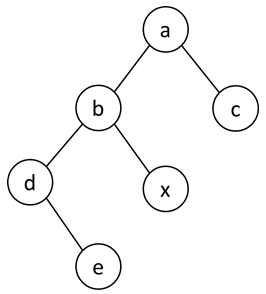
\includegraphics[width=2.60417in,height=2.87500in]{computerassets/E2AFE360B93D03349D89BFFBE4DFF49B.png}
\par\twoch{e、c}{e、a}{d、c}{\textcolor{red}{b、a}}
\begin{solution}首先求出中序遍历的顺序是debxac,可得结点x的左、右线索指向的结点分别是b和a。
\end{solution}
\question 若X是后序线索二叉树中的叶结点,且X存在左兄弟结点Y,则X的右线索指向的是(
)
\par\twoch{\textcolor{red}{X的父结点}}{以Y为根的子树的最左下结点}{X的左兄弟结点Y}{以Y为根的子树的最右下结点}
\begin{solution}由题目条件可知,X结点为叶子结点且有左兄弟,那么这个结点为右孩子结点,利用后序遍历的方式可知X结点的后继是其父结点,即X的右线索指向的是父结点。
\end{solution}
\question (中南大学,2005年)下面有关在中序线索树中查找指定节点的先序后继的问题时,下列说法错误是(
)
\par\fourch{当指定节点不是树叶时,若指定节点有左子女,则左子女是它的先序后继,若指定节点没有左子女,则右子女是它的先序后继}{当指定节点是树叶时,若指定节点是“某节点x”的左子树中按先序遍历列出的最后一个节点,且该节点x又有右子女,则指定节点的先序后继就是该的节点x的右子女}{当指定节点是树叶时,若指定节点虽然是“某节点x”的左子树中按先序遍历出的最后一个节点,但该节点x没有右子女,则指定节点没有先序后继}{\textcolor{red}{当指定节点是树叶时,若指定节点不是任何节点的左子树中按先序遍历列出的最后一个节点,则指定节点先序后继为根节点}}
\begin{solution}D选项中根节点必然为第一个访问的节点,所以无论如何,叶子节点的后继都不会是根节点
\end{solution}
\question (中山大学,2005年)线索二叉树与一般的二叉树相比,它更容易找到二叉树中节点的(
)
\par\twoch{左孩子}{右孩子}{双亲}{\textcolor{red}{前驱和后继}}
\begin{solution}线索二叉树的作用即方便查找前驱和后继
\end{solution}
\question (中国科学技术大学,2004年)一棵左右子树均不空的二叉树在先序线索化后,其中值为空的链域的个数是(
)
\par\twoch{0}{\textcolor{red}{1}}{2}{不确定}
\begin{solution}对于一棵左右子树均不空的二叉树,先序线索化后有一个值为空的链接,即最后一个输出节点的右指针
\end{solution}
